\subsection{Car detection with YOLOv2}

Welcome to your week 3 programming assignment. You will learn about object detection using the very powerful YOLO model. Many of the ideas in this assignment are described in the two YOLO papers: \href{https://arxiv.org/abs/1506.02640}{Redmon et al., 2016} and \href{https://arxiv.org/abs/1612.08242}{Redmon and Farhadi, 2016}.

You will learn to:
\begin{itemize}
\item Use object detection on a car detection dataset
\item Deal with bounding boxes
\end{itemize}

Run the following code to load the packages and dependencies that are going to be useful for your journey!
\begin{minted}{python}
import argparse
import os
import matplotlib.pyplot as plt
from matplotlib.pyplot import imshow
import scipy.io
import scipy.misc
import numpy as np
import pandas as pd
import PIL
import tensorflow as tf
from keras import backend as K
from keras.layers import Input, Lambda, Conv2D
from keras.models import load_model, Model
from yolo_utils import read_classes, read_anchors, generate_colors, preprocess_image, draw_boxes, scale_boxes
from yad2k.models.keras_yolo import yolo_head, yolo_boxes_to_corners, preprocess_true_boxes, yolo_loss, yolo_body

\end{minted}

{\textbf{Important Note}}: As you can see, we import Keras's backend as K. This means that to use a Keras function in this notebook, you will need to write: K.function(...).
\clearpage
\subsubsection{Problem Statement}

You are working on a self-driving car. As a critical component of this project, you'd like to first build a car detection system. To collect data, you've mounted a camera to the hood (meaning the front) of the car, which takes pictures of the road ahead every few seconds while you drive around.
\begin{figure}[h]
\begin{center}
\includegraphics[width=0.6\textwidth]{course4/self_driving_car}
\caption{Pictures taken from a car-mounted camera while driving around Silicon Valley}
\end{center}
\end{figure}

You've gathered all these images into a folder and have labelled them by drawing bounding boxes around every car you found. Here's an example of what your bounding boxes look like.
\begin{figure}[h]
\begin{center}
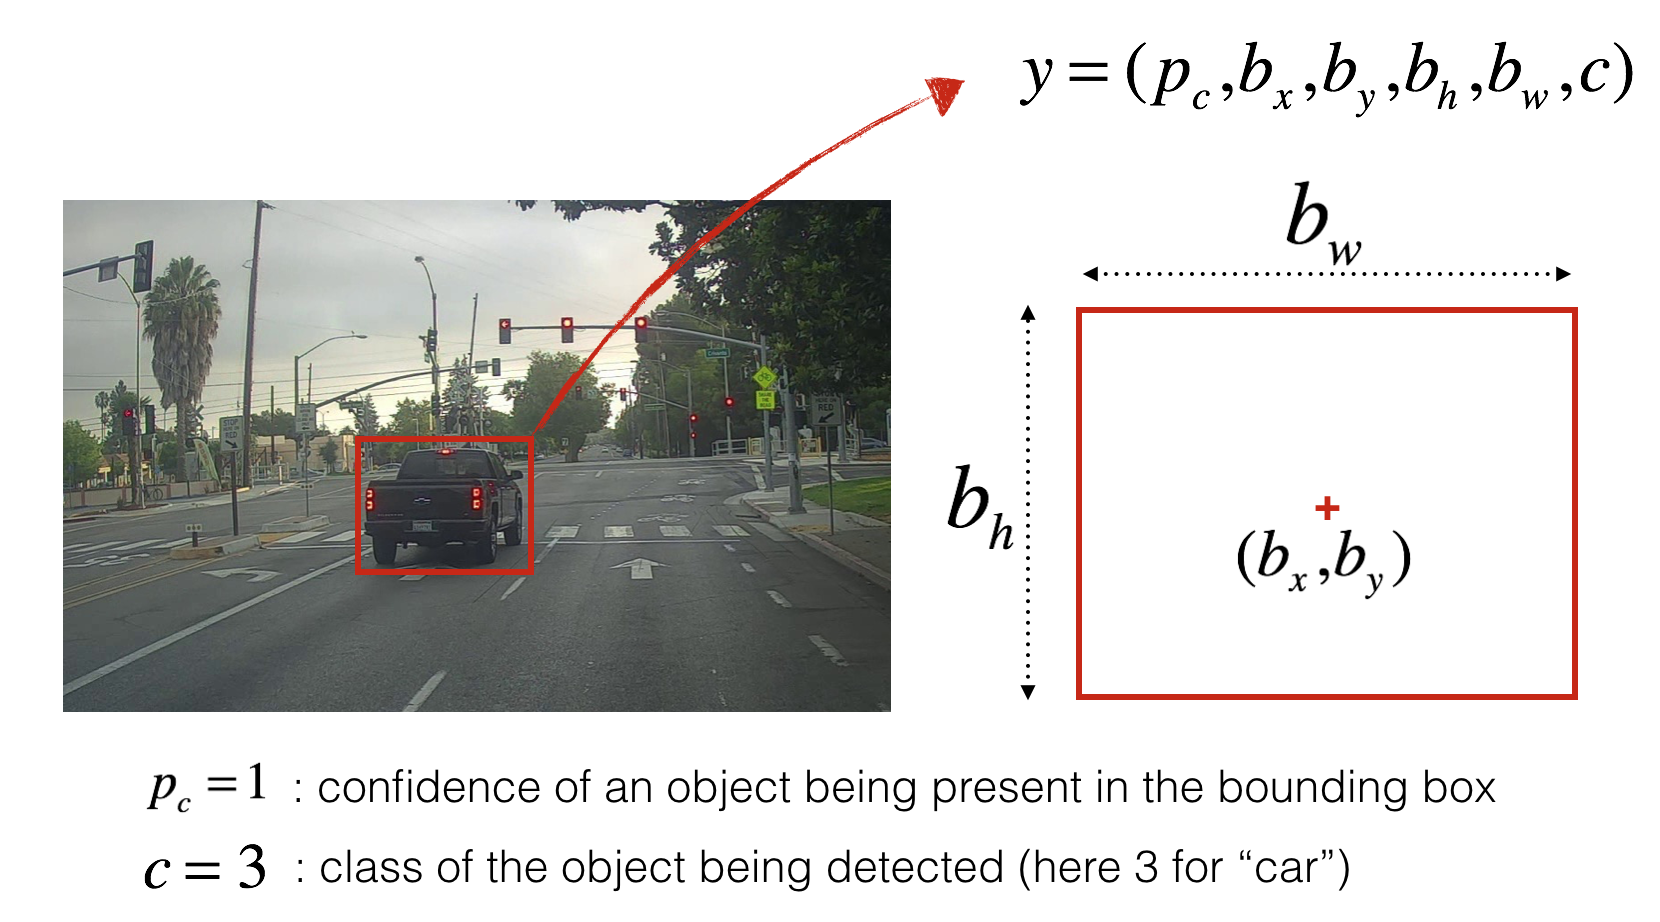
\includegraphics[width=0.8\textwidth]{course4/box_label}
\caption{Definition of a box}
\end{center}
\end{figure}

If you have 80 classes that you want YOLO to recognize, you can represent the class label  $c$  either as an integer from 1 to 80, or as an 80-dimensional vector (with 80 numbers) one component of which is 1 and the rest of which are 0. The video lectures had used the latter representation; in this notebook, we will use both representations, depending on which is more convenient for a particular step.

In this exercise, you will learn how YOLO works, then apply it to car detection. Because the YOLO model is very computationally expensive to train, we will load pre-trained weights for you to use.


\subsubsection{YOLO}
YOLO (``you only look once") is a popular algoritm because it achieves high accuracy while also being able to run in real-time. This algorithm ``only looks once" at the image in the sense that it requires only one forward propagation pass through the network to make predictions. After non-max suppression, it then outputs recognized objects together with the bounding boxes.

\subsubsubsection{Model details}

First things to know:
\begin{itemize}
\item The input is a batch of images of shape (m, 608, 608, 3)
\item The output is a list of bounding boxes along with the recognized classes. Each bounding box is represented by 6 numbers  $(p_c,b_x,b_y,b_h,b_w,c)$ as explained above. If you expand  $c$  into an 80-dimensional vector, each bounding box is then represented by 85 numbers.
\end{itemize}

We will use 5 anchor boxes. So you can think of the YOLO architecture as the following: IMAGE (m, 608, 608, 3) -> DEEP CNN -> ENCODING (m, 19, 19, 5, 85).

Lets look in greater detail at what this encoding represents.
\begin{figure}[h]
\begin{center}
\includegraphics[width=\textwidth]{course4/YOLO_architecture}
\caption{Encoding architecture for YOLO}
\label{YOLO_architecture}
\end{center}
\end{figure}

If the center/midpoint of an object falls into a grid cell, that grid cell is responsible for detecting that object.

Since we are using 5 anchor boxes, each of the 19 $\times$ 19 cells thus encodes information about 5 boxes. Anchor boxes are defined only by their width and height.

For simplicity, we will flatten the last two last dimensions of the shape (19, 19, 5, 85) encoding. So the output of the Deep CNN is (19, 19, 425).
\clearpage
\begin{figure}[h]
\begin{center}
\includegraphics[width=\textwidth]{course4/flatten_YOLO}
\caption{Flattening the last two last dimensions}
\end{center}
\end{figure}

Now, for each box (of each cell) we will compute the following elementwise product and extract a probability that the box contains a certain class.
\begin{figure}[h]
\begin{center}
\includegraphics[width=\textwidth]{course4/probability_extraction}
\caption{Find the class detected by each box}
\label{probability_extraction}
\end{center}
\end{figure}

Here's one way to visualize what YOLO is predicting on an image:
\begin{itemize}
\item For each of the 19$\times$19 grid cells, find the maximum of the probability scores (taking a max across both the 5 anchor boxes and across different classes).
\item Color that grid cell according to what object that grid cell considers the most likely.
\end{itemize}

Doing this results in this picture:
\begin{figure}[h]
\begin{center}
\includegraphics[width=0.5\textwidth]{course4/proba_map}
\caption{Each of the 19$\times$19 grid cells colored according to which class has the largest predicted probability in that cell}
\end{center}
\end{figure}

Note that this visualization isn't a core part of the YOLO algorithm itself for making predictions; it's just a nice way of visualizing an intermediate result of the algorithm.

Another way to visualize YOLO's output is to plot the bounding boxes that it outputs. Doing that results in a visualization like this:
\begin{figure}[h]
\begin{center}
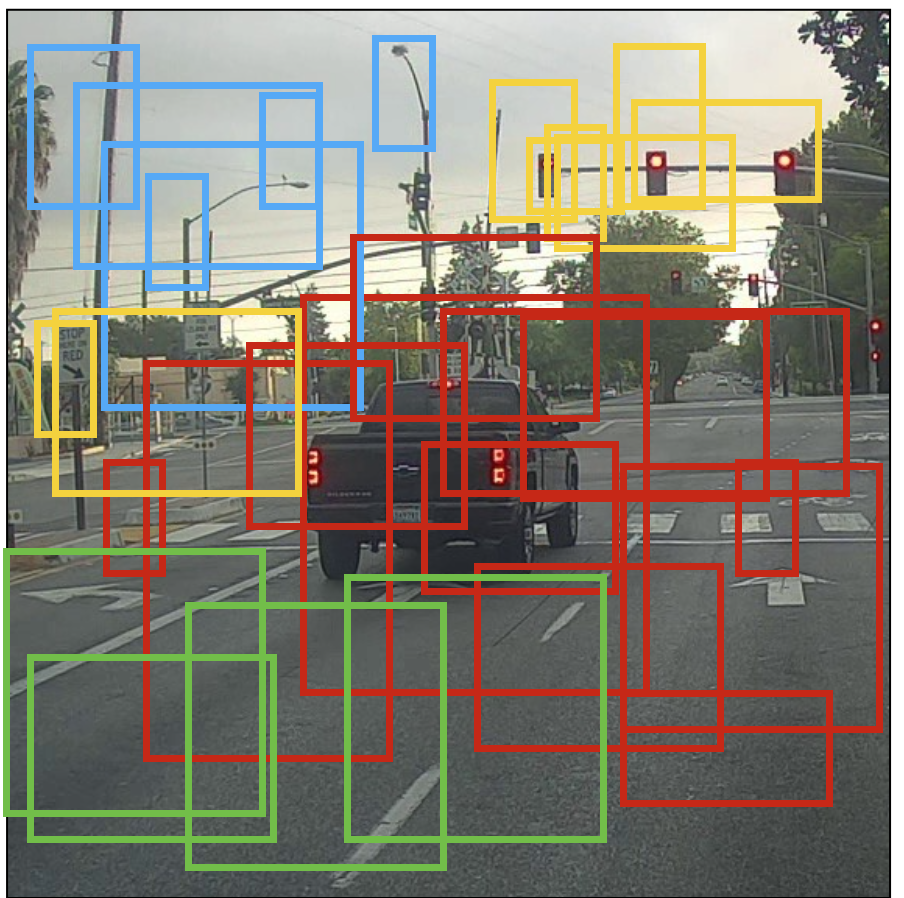
\includegraphics[width=0.5\textwidth]{course4/anchor_map}
\caption{Each cell gives you 5 boxes. In total, the model predicts: 19$\times$19$\times$5 = 1805 boxes just by looking once at the image (one forward pass through the network)! Different colors denote different classes. }
\end{center}
\end{figure}


In the figure above, we plotted only boxes that the model had assigned a high probability to, but this is still too many boxes. You'd like to filter the algorithm's output down to a much smaller number of detected objects. To do so, you'll use non-max suppression. Specifically, you'll carry out these steps:
\begin{itemize}
\item Get rid of boxes with a low score (meaning, the box is not very confident about detecting a class)
\item Select only one box when several boxes overlap with each other and detect the same object.
\end{itemize}


\subsubsubsection{Filtering with a threshold on class scores}

You are going to apply a first filter by thresholding. You would like to get rid of any box for which the class ``score" is less than a chosen threshold. 

The model gives you a total of 19$\times$19$\times$5$\times$85 numbers, with each box described by 85 numbers. It'll be convenient to rearrange the (19,19,5,85) (or (19,19,425)) dimensional tensor into the following variables: 
\begin{itemize} 
\item box\_confidence: tensor of shape $(19 \times 19, 5, 1)$ containing $p_c$ (confidence probability that there's some object) for each of the 5 boxes predicted in each of the 19$\times$19 cells.
\item boxes: tensor of shape $(19 \times 19, 5, 4)$ containing $(b_x, b_y, b_h, b_w)$ for each of the 5 boxes per cell.
\item box\_class\_probs: tensor of shape $(19 \times 19, 5, 80)$ containing the detection probabilities $(c_1, c_2, ... c_{80})$ for each of the 80 classes for each of the 5 boxes per cell.
\end{itemize}

{\textbf {Exercise}}: Implement yolo\_filter\_boxes().
\begin{itemize} 
\item[1.] Compute box scores by doing the elementwise product as described in Figure \ref{probability_extraction}. The following code may help you choose the right operator: 
\begin{minted}{python}
a = np.random.randn(19*19, 5, 1)
b = np.random.randn(19*19, 5, 80)
c = a * b # shape of c will be (19*19, 5, 80)
\end{minted}
\item[2.] For each box, find:
    \begin{itemize} 
    \item the index of the class with the maximum box score (\href{https://keras.io/backend/#argmax}{Hint}) (Be careful with what axis you choose; consider using axis=-1)
    \item the corresponding box score (\href{https://keras.io/backend/#max}{Hint}) (Be careful with what axis you choose; consider using axis=-1)
    \end{itemize}
\item[3.] Create a mask by using a threshold. As a reminder: ``([0.9, 0.3, 0.4, 0.5, 0.1] < 0.4)'' returns: ``[False, True, False, False, True]''. The mask should be True for the boxes you want to keep. 
\item[4.] Use TensorFlow to apply the mask to box\_class\_scores, boxes and box\_classes to filter out the boxes we don't want. You should be left with just the subset of boxes you want to keep. (\href{https://www.tensorflow.org/api_docs/python/tf/boolean_mask}{Hint})
\end{itemize}
Reminder: to call a Keras function, you should use ``K.function(...)''.

\begin{minted}{python}
# GRADED FUNCTION: yolo_filter_boxes
def yolo_filter_boxes(box_confidence, boxes, box_class_probs, threshold = .6):
    """Filters YOLO boxes by thresholding on object and class confidence.
    
    Arguments:
    box_confidence -- tensor of shape (19, 19, 5, 1)
    boxes -- tensor of shape (19, 19, 5, 4)
    box_class_probs -- tensor of shape (19, 19, 5, 80)
    threshold -- real value, if [ highest class probability score < threshold], then get rid of the corresponding box
    
    Returns:
    scores -- tensor of shape (None,), containing the class probability score for selected boxes
    boxes -- tensor of shape (None, 4), containing (b_x, b_y, b_h, b_w) coordinates of selected boxes
    classes -- tensor of shape (None,), containing the index of the class detected by the selected boxes
    
    Note: "None" is here because you don't know the exact number of selected boxes, as it depends on the threshold. 
    For example, the actual output size of scores would be (10,) if there are 10 boxes.
    """
    
    # Step 1: Compute box scores
    ### START CODE HERE ### (≈ 1 line)
    box_scores = box_confidence * box_class_probs
    ### END CODE HERE ###
    
    # Step 2: Find the box_classes thanks to the max box_scores, keep track of the corresponding score
    ### START CODE HERE ### (≈ 2 lines)
    box_classes = K.argmax(box_scores, axis=-1)
    box_class_scores = K.max(box_scores, axis=-1)
    ### END CODE HERE ###
    
    # Step 3: Create a filtering mask based on "box_class_scores" by using "threshold". The mask should have the
    # same dimension as box_class_scores, and be True for the boxes you want to keep (with probability >= threshold)
    ### START CODE HERE ### (≈ 1 line)
    filtering_mask = box_class_scores >= threshold
    ### END CODE HERE ###
    
    # Step 4: Apply the mask to scores, boxes and classes
    ### START CODE HERE ### (≈ 3 lines)
    scores = tf.boolean_mask(box_class_scores, filtering_mask)
    boxes = tf.boolean_mask(boxes, filtering_mask)
    classes = tf.boolean_mask(box_classes, filtering_mask)
    ### END CODE HERE ###
    
    return scores, boxes, classes
\end{minted}



\subsubsubsection{Non-max suppression}
Even after filtering by thresholding over the classes scores, you still end up a lot of overlapping boxes. A second filter for selecting the right boxes is called non-maximum suppression (NMS).
\begin{figure}[h]
\begin{center}
\includegraphics[width=0.8\textwidth]{course4/non-max-suppression}
\caption{In this example, the model has predicted 3 cars, but it's actually 3 predictions of the same car. Running non-max suppression (NMS) will select only the most accurate (highest probabiliy) one of the 3 boxes}
\end{center}
\end{figure}

Non-max suppression uses the very important function called {\textbf {``Intersection over Union"}}, or IoU.
\begin{figure}[h]
\begin{center}
\includegraphics[width=0.8\textwidth]{course4/iou}
\caption{Definition of ``Intersection over Union". }
\end{center}
\end{figure}




{\textbf {Exercise}}: Implement iou(). Some hints:

In this exercise only, we define a box using its two corners (upper left and lower right): (x1, y1, x2, y2) rather than the midpoint and height/width.
\begin{itemize}
\item To calculate the area of a rectangle you need to multiply its height (y2 - y1) by its width (x2 - x1)
\item You'll also need to find the coordinates (xi1, yi1, xi2, yi2) of the intersection of two boxes. Remember that:
\begin{itemize}
\item xi1 = maximum of the x1 coordinates of the two boxes
\item yi1 = maximum of the y1 coordinates of the two boxes
\item xi2 = minimum of the x2 coordinates of the two boxes
\item yi2 = minimum of the y2 coordinates of the two boxes
\end{itemize}
\end{itemize}

In this code, we use the convention that (0,0) is the top-left corner of an image, (1,0) is the upper-right corner, and (1,1) the lower-right corner.
\begin{minted}{python}
# GRADED FUNCTION: iou
def iou(box1, box2):
    """Implement the intersection over union (IoU) between box1 and box2
    
    Arguments:
    box1 -- first box, list object with coordinates (x1, y1, x2, y2)
    box2 -- second box, list object with coordinates (x1, y1, x2, y2)
    """

    # Calculate the (y1, x1, y2, x2) coordinates of the intersection of box1 and box2. Calculate its Area.
    ### START CODE HERE ### (≈ 5 lines)
    xi1 = max(box1[0],box2[0])
    yi1 = max(box1[1],box2[1])
    xi2 = min(box1[2],box2[2])
    yi2 = min(box1[3],box2[3])
    inter_area = (xi2 - xi1)*(yi2 - yi1)
    ### END CODE HERE ###    

    # Calculate the Union area by using Formula: Union(A,B) = A + B - Inter(A,B)
    ### START CODE HERE ### (≈ 3 lines)
    box1_area = (box1[2]-box1[0])*(box1[3]-box1[1])
    box2_area = (box2[2]-box2[0])*(box2[3]-box2[1])
    union_area =  box1_area + box2_area - inter_area
    ### END CODE HERE ###
    
    # compute the IoU
    ### START CODE HERE ### (≈ 1 line)
    iou = inter_area/union_area 
    ### END CODE HERE ###

    return iou
\end{minted}
\begin{minted}{python}
box1 = (2, 1, 4, 3)
box2 = (1, 2, 3, 4) 
print("iou = " + str(iou(box1, box2)))

#output
iou = 0.14285714285714285
\end{minted}


You are now ready to implement non-max suppression. The key steps are:
\begin{itemize}
\item Select the box that has the highest score.
\item Compute its overlap with all other boxes, and remove boxes that overlap it more than iou\_threshold.
\item Go back to step 1 and iterate until there's no more boxes with a lower score than the current selected box.
\end{itemize}

This will remove all boxes that have a large overlap with the selected boxes. Only the ``best" boxes remain.

{\textbf{Exercise}}: Implement yolo\_non\_max\_suppression() using TensorFlow. TensorFlow has two built-in functions that are used to implement non-max suppression (so you don't actually need to use your iou() implementation):
\begin{itemize}
\item \href{https://www.tensorflow.org/api_docs/python/tf/image/non_max_suppression}{tf.image.non\_max\_suppression()}
\item \href{https://www.tensorflow.org/api_docs/python/tf/gather}{K.gather()}
\end{itemize}

\begin{minted}{python}
# GRADED FUNCTION: yolo_non_max_suppression
def yolo_non_max_suppression(scores, boxes, classes, max_boxes = 10, iou_threshold = 0.5):
    """
    Applies Non-max suppression (NMS) to set of boxes
    
    Arguments:
    scores -- tensor of shape (None,), output of yolo_filter_boxes()
    boxes -- tensor of shape (None, 4), output of yolo_filter_boxes() that have been scaled to the image size (see later)
    classes -- tensor of shape (None,), output of yolo_filter_boxes()
    max_boxes -- integer, maximum number of predicted boxes you'd like
    iou_threshold -- real value, "intersection over union" threshold used for NMS filtering
    
    Returns:
    scores -- tensor of shape (, None), predicted score for each box
    boxes -- tensor of shape (4, None), predicted box coordinates
    classes -- tensor of shape (, None), predicted class for each box
    
    Note: The "None" dimension of the output tensors has obviously to be less than max_boxes. Note also that this
    function will transpose the shapes of scores, boxes, classes. This is made for convenience.
    """
    
    max_boxes_tensor = K.variable(max_boxes, dtype='int32')     # tensor to be used in tf.image.non_max_suppression()
    K.get_session().run(tf.variables_initializer([max_boxes_tensor])) # initialize variable max_boxes_tensor
    
    # Use tf.image.non_max_suppression() to get the list of indices corresponding to boxes you keep
    ### START CODE HERE ### (≈ 1 line)
    nms_indices = tf.image.non_max_suppression(boxes, scores, max_boxes, iou_threshold)
    ### END CODE HERE ###
    
    # Use K.gather() to select only nms_indices from scores, boxes and classes
    ### START CODE HERE ### (≈ 3 lines)
    scores = K.gather(scores, nms_indices)
    boxes =  K.gather(boxes, nms_indices)
    classes = K.gather(classes, nms_indices)
    ### END CODE HERE ###
    
    return scores, boxes, classes
\end{minted}






\subsubsubsection{Wrapping up the filtering}

It's time to implement a function taking the output of the deep CNN (the 19$\times$19$\times$5$\times$85 dimensional encoding) and filtering through all the boxes using the functions you've just implemented. 

{\textbf{Exercise}}: Implement ``yolo\_eval()'' which takes the output of the YOLO encoding and filters the boxes using score threshold and NMS. There's just one last implementational detail you have to know. There're a few ways of representing boxes, such as via their corners or via their midpoint and height/width. YOLO converts between a few such formats at different times, using the following functions (which we have provided): 

\begin{minted}{python}
boxes = yolo_boxes_to_corners(box_xy, box_wh) 
\end{minted}
which converts the yolo box coordinates (x,y,w,h) to box corners' coordinates (x1, y1, x2, y2) to fit the input of ``yolo\_filter\_boxes''
\begin{minted}{python}
boxes = scale_boxes(boxes, image_shape)
\end{minted}
YOLO's network was trained to run on 608$\times$608 images. If you are testing this data on a different size image--for example, the car detection dataset had 720$\times$1280 images--this step rescales the boxes so that they can be plotted on top of the original 720$\times$1280 image.  

Don't worry about these two functions; we'll show you where they need to be called.  

\begin{minted}{python}
# GRADED FUNCTION: yolo_eval
def yolo_eval(yolo_outputs, image_shape = (720., 1280.), max_boxes=10, score_threshold=.6, iou_threshold=.5):
    """
    Converts the output of YOLO encoding (a lot of boxes) to your predicted boxes along with their scores, box coordinates and classes.
    
    Arguments:
    yolo_outputs -- output of the encoding model (for image_shape of (608, 608, 3)), contains 4 tensors:
                box_confidence: tensor of shape (None, 19, 19, 5, 1)
                box_xy: tensor of shape (None, 19, 19, 5, 2)
                box_wh: tensor of shape (None, 19, 19, 5, 2)
                box_class_probs: tensor of shape (None, 19, 19, 5, 80)
    image_shape -- tensor of shape (2,) containing the input shape, in this notebook we use (608., 608.) (has to be float32 dtype)
    max_boxes -- integer, maximum number of predicted boxes you'd like
    score_threshold -- real value, if [ highest class probability score < threshold], then get rid of the corresponding box
    iou_threshold -- real value, "intersection over union" threshold used for NMS filtering
    
    Returns:
    scores -- tensor of shape (None, ), predicted score for each box
    boxes -- tensor of shape (None, 4), predicted box coordinates
    classes -- tensor of shape (None,), predicted class for each box
    """
    
    ### START CODE HERE ### 
    
    # Retrieve outputs of the YOLO model (≈1 line)
    box_confidence, box_xy, box_wh, box_class_probs = yolo_outputs

    # Convert boxes to be ready for filtering functions 
    boxes = yolo_boxes_to_corners(box_xy, box_wh)

    # Use one of the functions you've implemented to perform Score-filtering with a threshold of score_threshold (≈1 line)
    scores, boxes, classes = yolo_filter_boxes(box_confidence, boxes, box_class_probs, score_threshold)
    
    # Scale boxes back to original image shape.
    boxes = scale_boxes(boxes, image_shape)

    # Use one of the functions you've implemented to perform Non-max suppression with a threshold of iou_threshold (≈1 line)
    scores, boxes, classes = yolo_non_max_suppression(scores, boxes, classes, max_boxes, iou_threshold)
    
    ### END CODE HERE ###
    
    return scores, boxes, classes
\end{minted}


{\color{red}\textbf{Summary for YOLO}:
\begin{itemize}
\item Input image (608, 608, 3)
\item The input image goes through a CNN, resulting in a (19,19,5,85) dimensional output. 
\item After flattening the last two dimensions, the output is a volume of shape (19, 19, 425):
    \begin{itemize}
    \item Each cell in a 19$\times$19 grid over the input image gives 425 numbers. 
    \item 425 = 5 $\times$ 85 because each cell contains predictions for 5 boxes, corresponding to 5 anchor boxes, as seen in lecture. 
    \item 85 = 5 + 80 where 5 is because $(p_c, b_x, b_y, b_h, b_w)$ has 5 numbers, and and 80 is the number of classes we'd like to detect
    \end{itemize}
\item You then select only few boxes based on:
    \begin{itemize}
    \item Score-thresholding: throw away boxes that have detected a class with a score less than the threshold
    \item Non-max suppression: Compute the Intersection over Union and avoid selecting overlapping boxes
    \end{itemize}
\item This gives you YOLO's final output. 
\end{itemize}
}



\subsubsection{Test YOLO pretrained model on images}

In this part, you are going to use a pretrained model and test it on the car detection dataset. As usual, you start by creating a session to start your graph. Run the following cell.
\begin{minted}{python}
sess = K.get_session()
\end{minted}


\subsubsubsection{Defining classes, anchors and image shape}

Recall that we are trying to detect 80 classes, and are using 5 anchor boxes. We have gathered the information about the 80 classes and 5 boxes in two files ``coco\_classes.txt" and "yolo\_anchors.txt". Let's load these quantities into the model by running the next code.

The car detection dataset has 720$\times$1280 images, which we've pre-processed into 608$\times$608 images.
\begin{minted}{python}
class_names = read_classes("model_data/coco_classes.txt")
anchors = read_anchors("model_data/yolo_anchors.txt")
image_shape = (720., 1280.)    
\end{minted}

\subsubsubsection{Loading a pretrained model}
Training a YOLO model takes a very long time and requires a fairly large dataset of labelled bounding boxes for a large range of target classes. You are going to load an existing pretrained Keras YOLO model stored in ``yolo.h5". (These weights come from the official YOLO website, and were converted using a function written by Allan Zelener. References are at the end of this assignment. Technically, these are the parameters from the ``YOLOv2" model, but we will more simply refer to it as ``YOLO" in this assignment.) Run the code below to load the model from this file.
\begin{minted}{python}
yolo_model = load_model("model_data/yolo.h5")
\end{minted}

This loads the weights of a trained YOLO model. Here's a summary of the layers your model contains.
\begin{minted}{python}
yolo_model.summary()

#output
__________________________________________________________________
Layer (type)                     Output Shape          Param #     Connected to                     
==================================================================
input_1 (InputLayer)             (None, 608, 608, 3)   0                                            
__________________________________________________________________
conv2d_1 (Conv2D)                (None, 608, 608, 32)  864         input_1[0][0]                    
__________________________________________________________________
batch_normalization_1 (BatchNorm (None, 608, 608, 32)  128         conv2d_1[0][0]                   
__________________________________________________________________
......
__________________________________________________________________
batch_normalization_22 (BatchNor (None, 19, 19, 1024)  4096        conv2d_22[0][0]                  
__________________________________________________________________
leaky_re_lu_22 (LeakyReLU)       (None, 19, 19, 1024)  0           batch_normalization_22[0][0]     
__________________________________________________________________
conv2d_23 (Conv2D)               (None, 19, 19, 425)   435625      leaky_re_lu_22[0][0]             
==================================================================
Total params: 50,983,561
Trainable params: 50,962,889
Non-trainable params: 20,672
__________________________________________________________________
\end{minted}

{\textbf{Reminder}}: this model converts a preprocessed batch of input images (shape: (m, 608, 608, 3)) into a tensor of shape (m, 19, 19, 5, 85) as explained in Figure \ref{YOLO_architecture}.


\subsubsubsection{Convert output of the model to usable bounding box tensors}
The output of yolo\_model is a (m, 19, 19, 5, 85) tensor that needs to pass through non-trivial processing and conversion. The following code does that for you.
\begin{minted}{python}
yolo_outputs = yolo_head(yolo_model.output, anchors, len(class_names))
\end{minted}

You added yolo\_outputs to your graph. This set of 4 tensors is ready to be used as input by your yolo\_eval function.


\subsubsubsection{Filtering boxes}

yolo\_outputs gave you all the predicted boxes of yolo\_model in the correct format. You're now ready to perform filtering and select only the best boxes. Lets now call yolo\_eval, which you had previously implemented, to do this.
\begin{minted}{python}
scores, boxes, classes = yolo_eval(yolo_outputs, image_shape)
\end{minted}



\subsubsubsection{Run the graph on an image}

Let the fun begin. You have created a (sess) graph that can be summarized as follows:
\begin{itemize}
\item[1.] yolo\_model.input is given to yolo\_model. The model is used to compute the output yolo\_model.output
\item[2.] yolo\_model.output is processed by yolo\_head. It gives you yolo\_outputs
\item[3.] yolo\_outputs goes through a filtering function, yolo\_eval. It outputs your predictions: scores, boxes, classes
\end{itemize}

{\textbf{Exercise}}: Implement predict() which runs the graph to test YOLO on an image. You will need to run a TensorFlow session, to have it compute scores, boxes, classes.

The code below also uses the following function:
\begin{minted}{python}
image, image_data = preprocess_image("images/" + image_file, model_image_size = (608, 608))
\end{minted}
which outputs:
\begin{itemize}
\item image: a python (PIL) representation of your image used for drawing boxes. You won't need to use it.
\item image\_data: a numpy-array representing the image. This will be the input to the CNN.
\end{itemize}

{\textbf{Important note}}: when a model uses BatchNorm (as is the case in YOLO), you will need to pass an additional placeholder in the feed\_dict \{K.learning\_phase(): 0\}.
\begin{minted}{python}
def predict(sess, image_file):
    """
    Runs the graph stored in "sess" to predict boxes for "image_file". Prints and plots the preditions.
    
    Arguments:
    sess -- your tensorflow/Keras session containing the YOLO graph
    image_file -- name of an image stored in the "images" folder.
    
    Returns:
    out_scores -- tensor of shape (None, ), scores of the predicted boxes
    out_boxes -- tensor of shape (None, 4), coordinates of the predicted boxes
    out_classes -- tensor of shape (None, ), class index of the predicted boxes
    
    Note: "None" actually represents the number of predicted boxes, it varies between 0 and max_boxes. 
    """

    # Preprocess your image
    image, image_data = preprocess_image("images/" + image_file, model_image_size = (608, 608))

    # Run the session with the correct tensors and choose the correct placeholders in the feed_dict.
    # You'll need to use feed_dict={yolo_model.input: ... , K.learning_phase(): 0})
    ### START CODE HERE ### (≈ 1 line)
    out_scores, out_boxes, out_classes = sess.run([scores, boxes, classes],feed_dict={yolo_model.input: image_data, K.learning_phase(): 0})
    ### END CODE HERE ###

    # Print predictions info
    print('Found {} boxes for {}'.format(len(out_boxes), image_file))
    # Generate colors for drawing bounding boxes.
    colors = generate_colors(class_names)
    # Draw bounding boxes on the image file
    draw_boxes(image, out_scores, out_boxes, out_classes, class_names, colors)
    # Save the predicted bounding box on the image
    image.save(os.path.join("out", image_file), quality=90)
    # Display the results in the notebook
    output_image = scipy.misc.imread(os.path.join("out", image_file))
    imshow(output_image)
    
    return out_scores, out_boxes, out_classes
\end{minted}

\begin{minted}{python}
out_scores, out_boxes, out_classes = predict(sess, "test.jpg")
#output
Found 7 boxes for test.jpg
car 0.60 (925, 285) (1045, 374)
car 0.66 (706, 279) (786, 350)
bus 0.67 (5, 266) (220, 407)
car 0.70 (947, 324) (1280, 705)
car 0.74 (159, 303) (346, 440)
car 0.80 (761, 282) (942, 412)
car 0.89 (367, 300) (745, 648)
\end{minted}
\clearpage
\begin{figure}[h]
\begin{center}
\includegraphics[width=0.5\textwidth]{course4/test_YOLO}
\end{center}
\end{figure}


The model you've just run is actually able to detect 80 different classes listed in ``coco\_classes.txt". To test the model on your own images:
\begin{itemize}
\item[1.] Click on ``File" in the upper bar of this notebook, then click ``Open" to go on your Coursera Hub.
\item[2.] Add your image to this Jupyter Notebook's directory, in the ``images" folder
\item[3.] Write your image's name in the code above code
\item[4.] Run the code and see the output of the algorithm!
\end{itemize}

If you were to run your session in a for loop over all your images. 

\clearpage

\noindent{\color{red}\textbf{What you should remember}:
\begin{itemize}
\item YOLO is a state-of-the-art object detection model that is fast and accurate
\item It runs an input image through a CNN which outputs a 19$\times$19$\times$5$\times$85 dimensional volume.
\item The encoding can be seen as a grid where each of the 19$\times$19 cells contains information about 5 boxes.
\item You filter through all the boxes using non-max suppression. Specifically:
\begin{itemize}
\item Score thresholding on the probability of detecting a class to keep only accurate (high probability) boxes
\item Intersection over Union (IoU) thresholding to eliminate overlapping boxes
\end{itemize}
\item Because training a YOLO model from randomly initialized weights is non-trivial and requires a large dataset as well as lot of computation, we used previously trained model parameters in this exercise. If you wish, you can also try fine-tuning the YOLO model with your own dataset, though this would be a fairly non-trivial exercise.
\end{itemize}
}


\noindent{\textbf{References}}: The ideas presented in this notebook came primarily from the two YOLO papers. The implementation here also took significant inspiration and used many components from Allan Zelener's github repository. The pretrained weights used in this exercise came from the official YOLO website.
\begin{itemize}
\item Joseph Redmon, Santosh Divvala, Ross Girshick, Ali Farhadi - \href{https://arxiv.org/abs/1506.02640)}{You Only Look Once: Unified, Real-Time Object Detection}(2015)
\item Joseph Redmon, Ali Farhadi - \href{https://arxiv.org/abs/1612.08242}{YOLO9000: Better, Faster, Stronger} (2016)
\item Allan Zelener - \href{https://github.com/allanzelener/YAD2K}{YAD2K: Yet Another Darknet 2 Keras}
\item The official YOLO website:\url{https://pjreddie.com/darknet/yolo/}
\end{itemize}
\clearpage